\documentclass[final]{beamer}

\usepackage[scale=1.24]{beamerposter}

\usetheme{confposter}

\setbeamercolor{block title}{fg=ngreen,bg=white}
\setbeamercolor{block body}{fg=black,bg=white}
\setbeamercolor{block alerted title}{fg=white,bg=dblue!70}
\setbeamercolor{block alerted body}{fg=black,bg=dblue!10}

\newlength{\sepwid}
\newlength{\onecolwid}
\newlength{\twocolwid}
\newlength{\threecolwid}
\setlength{\paperwidth}{48in}
\setlength{\paperheight}{36in}
\setlength{\sepwid}{0.024\paperwidth}
\setlength{\onecolwid}{0.22\paperwidth}
\setlength{\twocolwid}{0.464\paperwidth}
\setlength{\threecolwid}{0.708\paperwidth}
\setlength{\topmargin}{-0.5in}

\usepackage{graphicx}
\usepackage{booktabs}
\usepackage{xcolor}
\usepackage{amsmath}

\definecolor{ngreen}{RGB}{34,139,34}
\definecolor{dblue}{RGB}{0,0,139}
\definecolor{titletextcolor}{RGB}{50,50,50}
\definecolor{secondarycolor}{RGB}{100,100,100}
\definecolor{primarycolor}{RGB}{0,0,0}

\DeclareMathOperator*{\argmax}{argmax}
\DeclareMathOperator*{\argmin}{argmin}

%----------------------------------------------------------------------------------------
% META INFORMATION
%----------------------------------------------------------------------------------------

\title[Word Translation Without Parallel Data]{Word Translation Without Parallel Data (2018)}
\author[ ]{\textcolor{secondarycolor}{Poster by: A. Puigdemont Monllor, J. Ciesko}}
\institute[FI MU]{\textcolor{primarycolor}{Faculty of Informatics, Masaryk University}}
\date{\textcolor{primarycolor}{November 11, 2024}}

%----------------------------------------------------------------------------------------

\begin{document}

\addtobeamertemplate{block end}{}{\vspace*{2ex}}
\addtobeamertemplate{block alerted end}{}{\vspace*{2ex}}
\setlength{\belowcaptionskip}{2ex}
\setlength\belowdisplayshortskip{2ex}

\begin{frame}[t]

\begin{columns}[t]

\begin{column}{\sepwid}\end{column}

\begin{column}{\onecolwid}

%----------------------------------------------------------------------------------------
%	OBJECTIVES
%----------------------------------------------------------------------------------------

\begin{alertblock}{Objectives} %Title of block
\begin{itemize}
    \item Achieve word translation without using parallel data by aligning independently trained monolingual embeddings.
    \item Develop an adversarial training method to align embedding spaces.
\end{itemize}
\end{alertblock}

%----------------------------------------------------------------------------------------
%	INTRODUCTION
%----------------------------------------------------------------------------------------

\begin{block}{Model Overview}
    \textbf{Embedding Spaces and Translation Mapping}
    \begin{itemize}
        \item Two sets of word embeddings \( X \) (source) and \( Y \) (target) are used, trained on monolingual data.
        \item Embedding spaces \( X \) and \( Y \) do \textbf{not need to be of the same dimension.}
        \item Objective: Find a linear mapping \( W \) that aligns translations in a shared space by minimizing:
        \begin{equation}
            W^* = \argmin_{W} || W X - Y ||_F
        \end{equation}
        \item Translation for a source word \( s \) is done by maximizing cosine similarity:
        \begin{equation}
            t = \argmax_{t} \cos(W x_s, y_t)
        \end{equation}
    \end{itemize}
\end{block}

%----------------------------------------------------------------------------------------
%	ILLUSTRATION
%----------------------------------------------------------------------------------------

\begin{block}{Method Illustration}
\begin{center}
    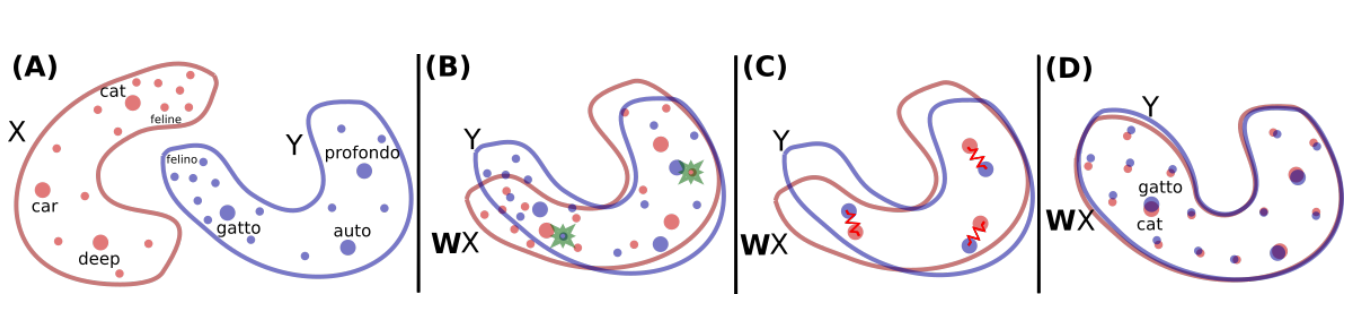
\includegraphics[width=0.9\linewidth]{figures/figure1.png}
\end{center}
\small
\textit{(A) Embeddings of English (red, \(X\)) and Italian (blue, \(Y\)), showing word frequency. (B) Adversarial training aligns \(X\) and \(Y\) via \(W\). (C) Procrustes refinement using frequent word anchors. (D) CSLS adjusts dense region distances, enhancing word alignment.}
\end{block}

\end{column} 

\begin{column}{\sepwid}\end{column} 

\begin{column}{twocolwid}

\begin{columns}[t,totalwidth=\twocolwid]

\begin{column}{\onecolwid}

%----------------------------------------------------------------------------------------
%	METHODS
%----------------------------------------------------------------------------------------

\begin{block}{Adversarial Training}
    \textbf{Domain-Adversarial Approach}
    \begin{itemize}
        \item Domain-adversarial training aligns \( WX \) and \( Y \) without cross-lingual supervision.
        \item A \textbf{discriminator} is trained to classify embeddings as source (transformed \( WX \)) or target (\( Y \)):
        \begin{equation}
            L_D(\theta_D | W) = - \frac{1}{n} \sum_{i=1}^n \log P_{\theta_D}(source = 1 | W x_i) - \frac{1}{m} \sum_{i=1}^m \log P_{\theta_D}(source = 0 | y_i)
        \end{equation}
        \item Mapping \( W \) is optimized to confuse the discriminator by minimizing the following:
        \begin{equation}
            L_W(W | \theta_D) = - \frac{1}{n} \sum_{i=1}^n \log P_{\theta_D}(source = 0 | W x_i) - \frac{1}{m} \sum_{i=1}^m \log P_{\theta_D}(source = 1 | y_i)
        \end{equation}
    \end{itemize}
\end{block}

\end{column}

\begin{column}{\onecolwid}

%----------------------------------------------------------------------------------------
%	REFINEMENT PROCEDURE
%----------------------------------------------------------------------------------------

\begin{block}{Refinement Procedure with Procrustes}
    \textbf{Refining the Mapping}
    \begin{itemize}
        \item Initial mapping \( W \) aligns well but struggles with rare words.
        \item Procrustes (orthogonal refinement) improves accuracy by minimizing:
        \begin{equation}
            W^* = \argmin_{W \in O_d(\mathbb{R})} || W X - Y ||_F
        \end{equation}
        \item This method iteratively aligns frequent words as anchors and is applied for a high-quality dictionary.
    \end{itemize}
\end{block}

\end{column} 

\end{columns} 

%----------------------------------------------------------------------------------------
%	CSLS
%----------------------------------------------------------------------------------------

\begin{block}{Cross-Domain Similarity Local Scaling (CSLS)}
    \textbf{Improving Nearest Neighbor Matching}
    \begin{itemize}
        \item CSLS reduces the effect of “hubs” in dense areas of the embedding space, where some vectors appear as nearest neighbors for many others.
        \item The CSLS similarity measure is:
        \begin{equation}
            CSLS(W x_s, y_t) = 2 \cos(W x_s, y_t) - r_T(W x_s) - r_S(y_t)
        \end{equation}
        Where:
        \begin{equation}
            r_T(W x_s) = \frac{1}{K} \sum_{y_t \in N_T(W x_s)} \cos(W x_s, y_t)
        \end{equation}
        \begin{equation}
            r_S(y_t) = \frac{1}{K} \sum_{x_s \in N_S(y_t)} \cos(x_s, y_t)
        \end{equation}
        \item CSLS adjusts similarity based on neighboring word density, enhancing translation accuracy.
    \end{itemize}
\end{block}

\end{column} 

\begin{column}{\sepwid}\end{column} 

\begin{column}{\onecolwid} 

%----------------------------------------------------------------------------------------
%	REFERENCES AND CONTACT
%----------------------------------------------------------------------------------------

\begin{block}{References}
\small
Mikolov, T., et al. (2013). Distributed Representations of Words and Phrases and Their Compositionality. *NeurIPS*.\\
Goodfellow, I., et al. (2014). Generative Adversarial Nets. *NeurIPS*.
...
\end{block}


\end{column}

\begin{column}{\sepwid}\end{column}

\end{columns}
\end{frame}
\end{document}
